\documentclass[10.5pt
%,draft
]{article}


\usepackage{ctex}
\usepackage{graphicx}
\usepackage{amsmath}
\usepackage{xcolor}
\usepackage{physics}
\usepackage{hyperref}
\hypersetup{
    colorlinks=true,
    linkcolor=Blue4Link,
    filecolor=magenta,      
    urlcolor=cyan,
    pdfauthor=徐均益
    }
\definecolor{Blue4Link}{RGB}{46,49,146}
\definecolor{myOrange}{RGB}{178,76,0}
\definecolor{green4eye}{RGB}{0,120,2}%
\definecolor{blue4eye}{RGB}{1,126,218}%
\definecolor{cyan4eye}{RGB}{31,186,190}%
\definecolor{myhighlight}{RGB}{255,214,161}
\definecolor{mybackground}{RGB}{204,232,207}
\usepackage{geometry}
\usepackage{natbib}
\usepackage{subcaption}

\renewcommand{\refname}{参考文献}
\renewcommand{\figurename}{图}
\renewcommand{\abstractname}{摘要}

\def\due{2023 年 4 月 26 日周一 8:40}
\def\Term{2023 年春季}
\def\Course{磁流体力学的数值模拟方法}

\title{一维气体激波管问题 --- 第 3 次作业\footnote{\Term\Course}}

\author{徐均益\footnote{ID: SA22214015 Email: jyxu@mail.ustc.edu.cn}
  \and
  余航\footnote{ID: SA22168021 Email: yh131996@mail.ustc.edu.cn}
  \and
  陈宇韬\footnote{ID: SA22214014 Email: chenyut@mail.ustc.edu.cn}
}

\date{%
\scriptsize%
%CAS Key Laboratory for Basic Plasma Physics, School of Earth and Space Sciences,
%\\
%University of Science and Technology of China, Hefei, Anhui 230026, China
中国科学技术大学核科学技术学院, 合肥 230026 \\
中国科学技术大学物质科学研究院等离子所, 合肥 230026
%
}

\begin{document}

\maketitle

\begin{abstract}
讨论一维气体激波管问题的有限差分数值解法, 结合理论分析讨论该方程的物理解和数值解的特性,
分析流体中不同波模的物理和数值特性, 请在 \textbf{\due} 前完成并提交. 

\end{abstract}

\section{引言}


\section{方程和初始条件}
考察一维多方气体 Euler 方程 \citep{Jeffrey1964}
\begin{align}
\frac{\partial w}{\partial t} + \frac{\partial f(w)}{\partial
x}= 0,\label{Eqn:Euler}
\end{align}
的 Riemann 问题 (一维气体激波管问题)
\begin{align}
w(x,t)|_{t=0} = \left\{ \begin{array}{ll}
W_L, & \quad x < 0 \\
W_R, & \quad x > 0
\end{array} \right.
\end{align}
其中
\begin{align}
w =& \left[\begin{array}{c}
\rho\\
m\\
E
\end{array}\right],
\\
f(w) =& u w + \left[\begin{array}{c}
0\\
p\\
p u
\end{array}\right] = \left[\begin{array}{c}
m
\\
(\gamma - 1) E + \frac{3 - \gamma}{2} \frac{m^2}{\rho}
\\
(\gamma E - \frac{\gamma - 1}{2} \frac{m^2}{\rho}) \frac{m}{\rho}
\end{array}\right],
\\
m =& \rho u,
\\
p =& (\gamma - 1)(E - \frac{1}{2} \rho u^2).
\end{align}
这里, $\rho$, $u$, $p$ 和 $E$ 分别是密度, 速度, 压力和总能量. 为和经典数值计算结果比较, 取文献 \citet{Harten1983} 中的值, 即 $\gamma=1.4$, 和
\begin{align}
    W_L = \left[\begin{array}{l}
    0.445\\
    0.311\\
    8.928
    \end{array}\right], \quad W_R = \left[\begin{array}{l}
    0.5\\
    0\\
    1.4275
    \end{array}\right]
\end{align}
设计两到三种有限差分格式, 编程进行数值计算, 给出图形, 比较和讨论结果. 或者, 利用附件中的 Excel 表格, 生成别的初值条件及解, 对流体力学中的间断问题进行数值计算并作进一步的讨论.

作为参考, 这里给出三个算例, CFL 系数均取 0.5, $t=0.14$ 时刻的数值的计算结果. 迎风格式, 261 网格的数据如图~\ref{Fig:Upwind},
TVD (Total Variation Diminishing) 格式 \citep{vanLeer1974,Harten1983}, 133 网格的数据如图~\ref{Fig:vanLeerA}, 以及 TVD 格式, 261
网格的数据如图~\ref{Fig:vanLeerB}. 供大家参考.

\begin{figure}
\begin{center}
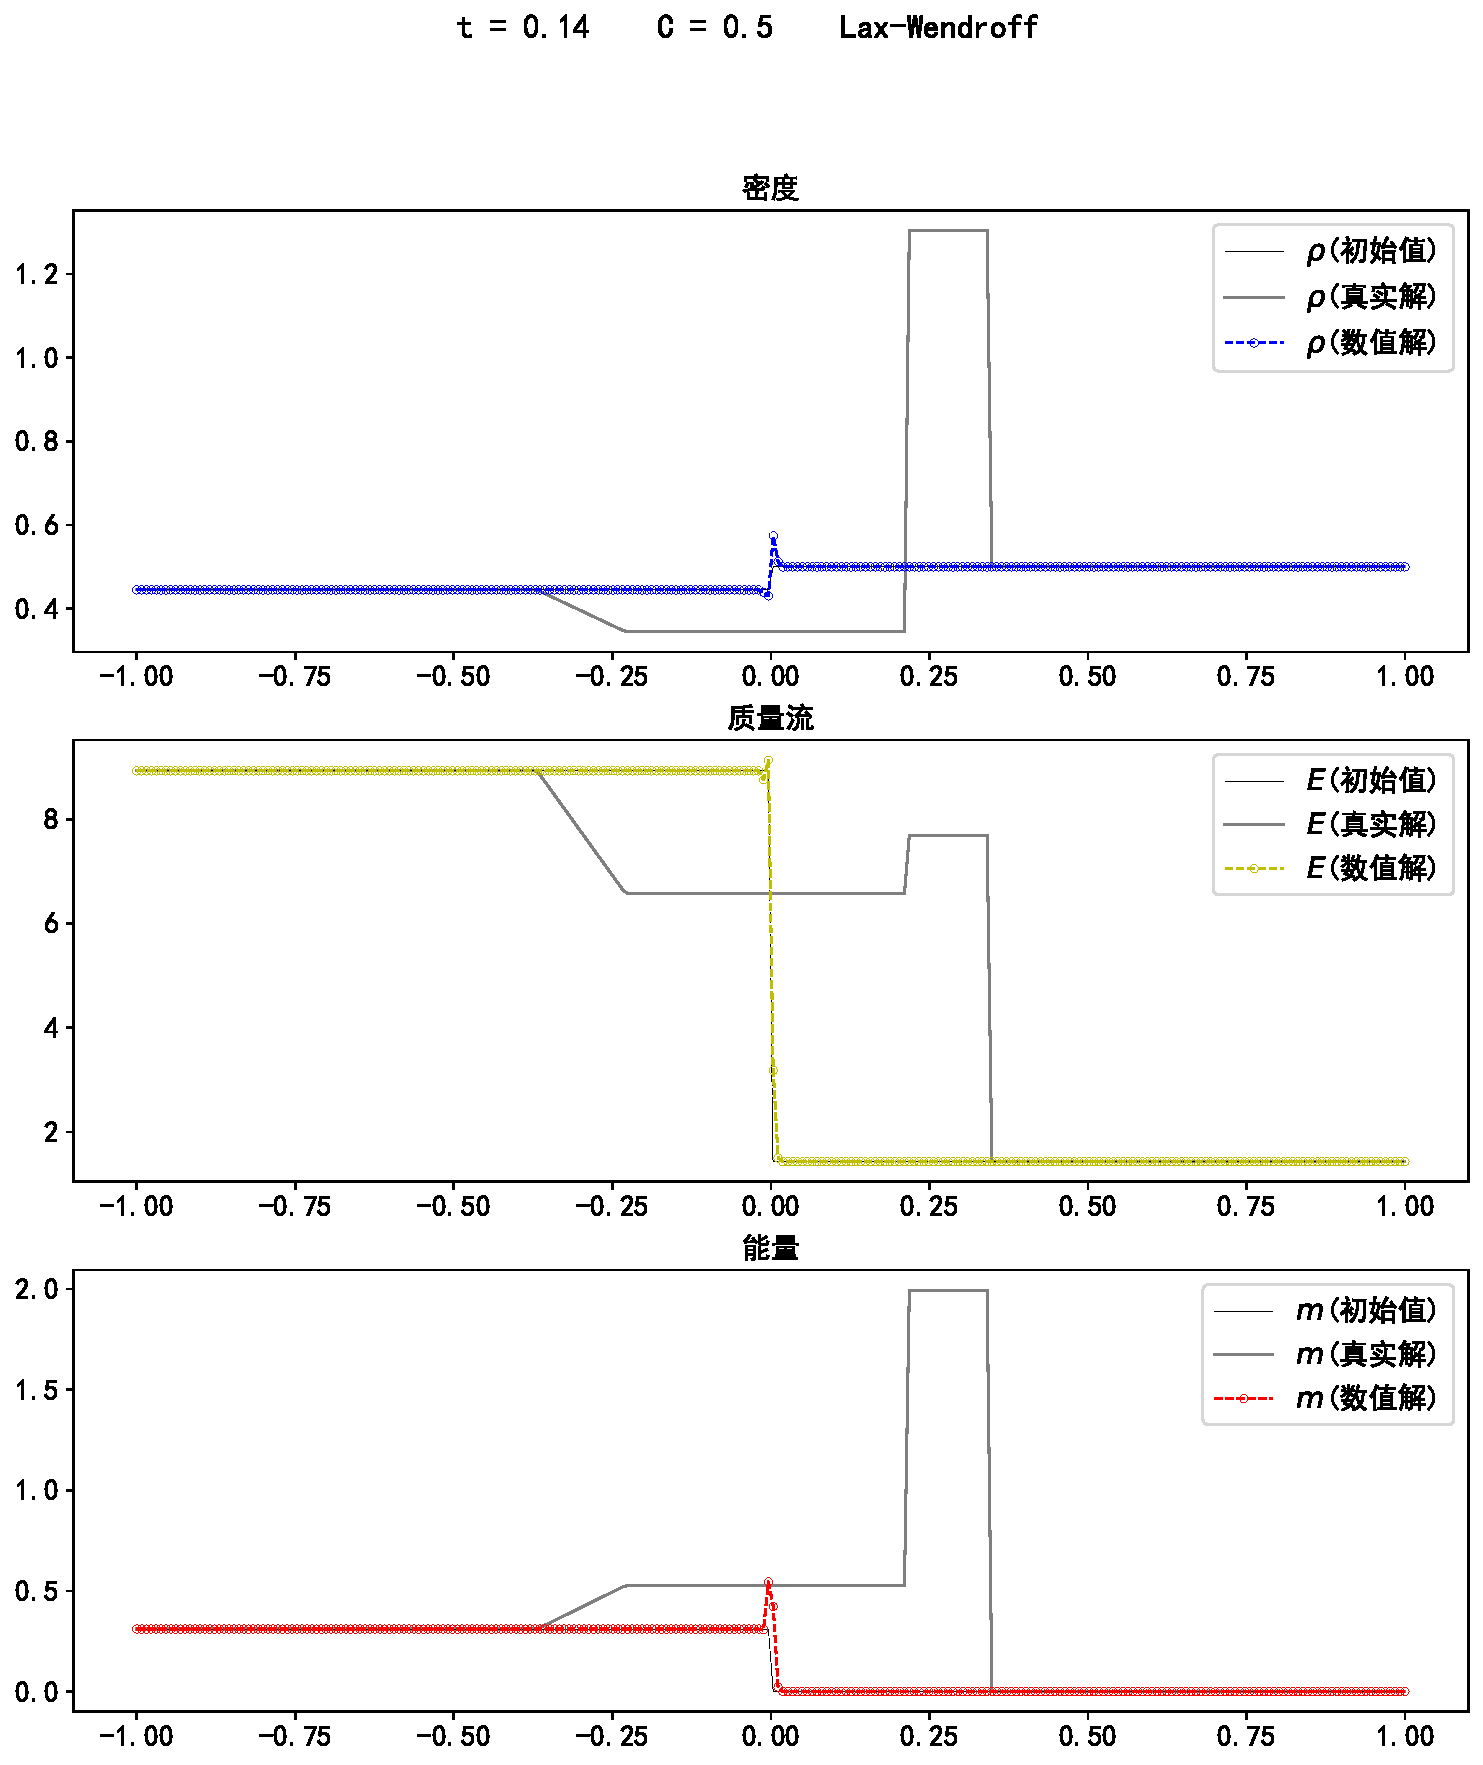
\includegraphics[width=.85\textwidth]{figures/lax_wendroff261.pdf}
\caption{Lax-Wendroff 格式计算结果, 网格点数为 261. \textbf{从上到下分别是密度 $\rho$, 能量 $E$ 和质量流 $m = \rho u$.}
其中点线是初值, 虚线 (上面的数据点用符号 $\circ$ 标注) 是 $t=0.14$ 时的数值结果, 实线是对应的真实解.}\label{Fig:Upwind}
\end{center}

\end{figure}
\begin{figure}
\begin{center}
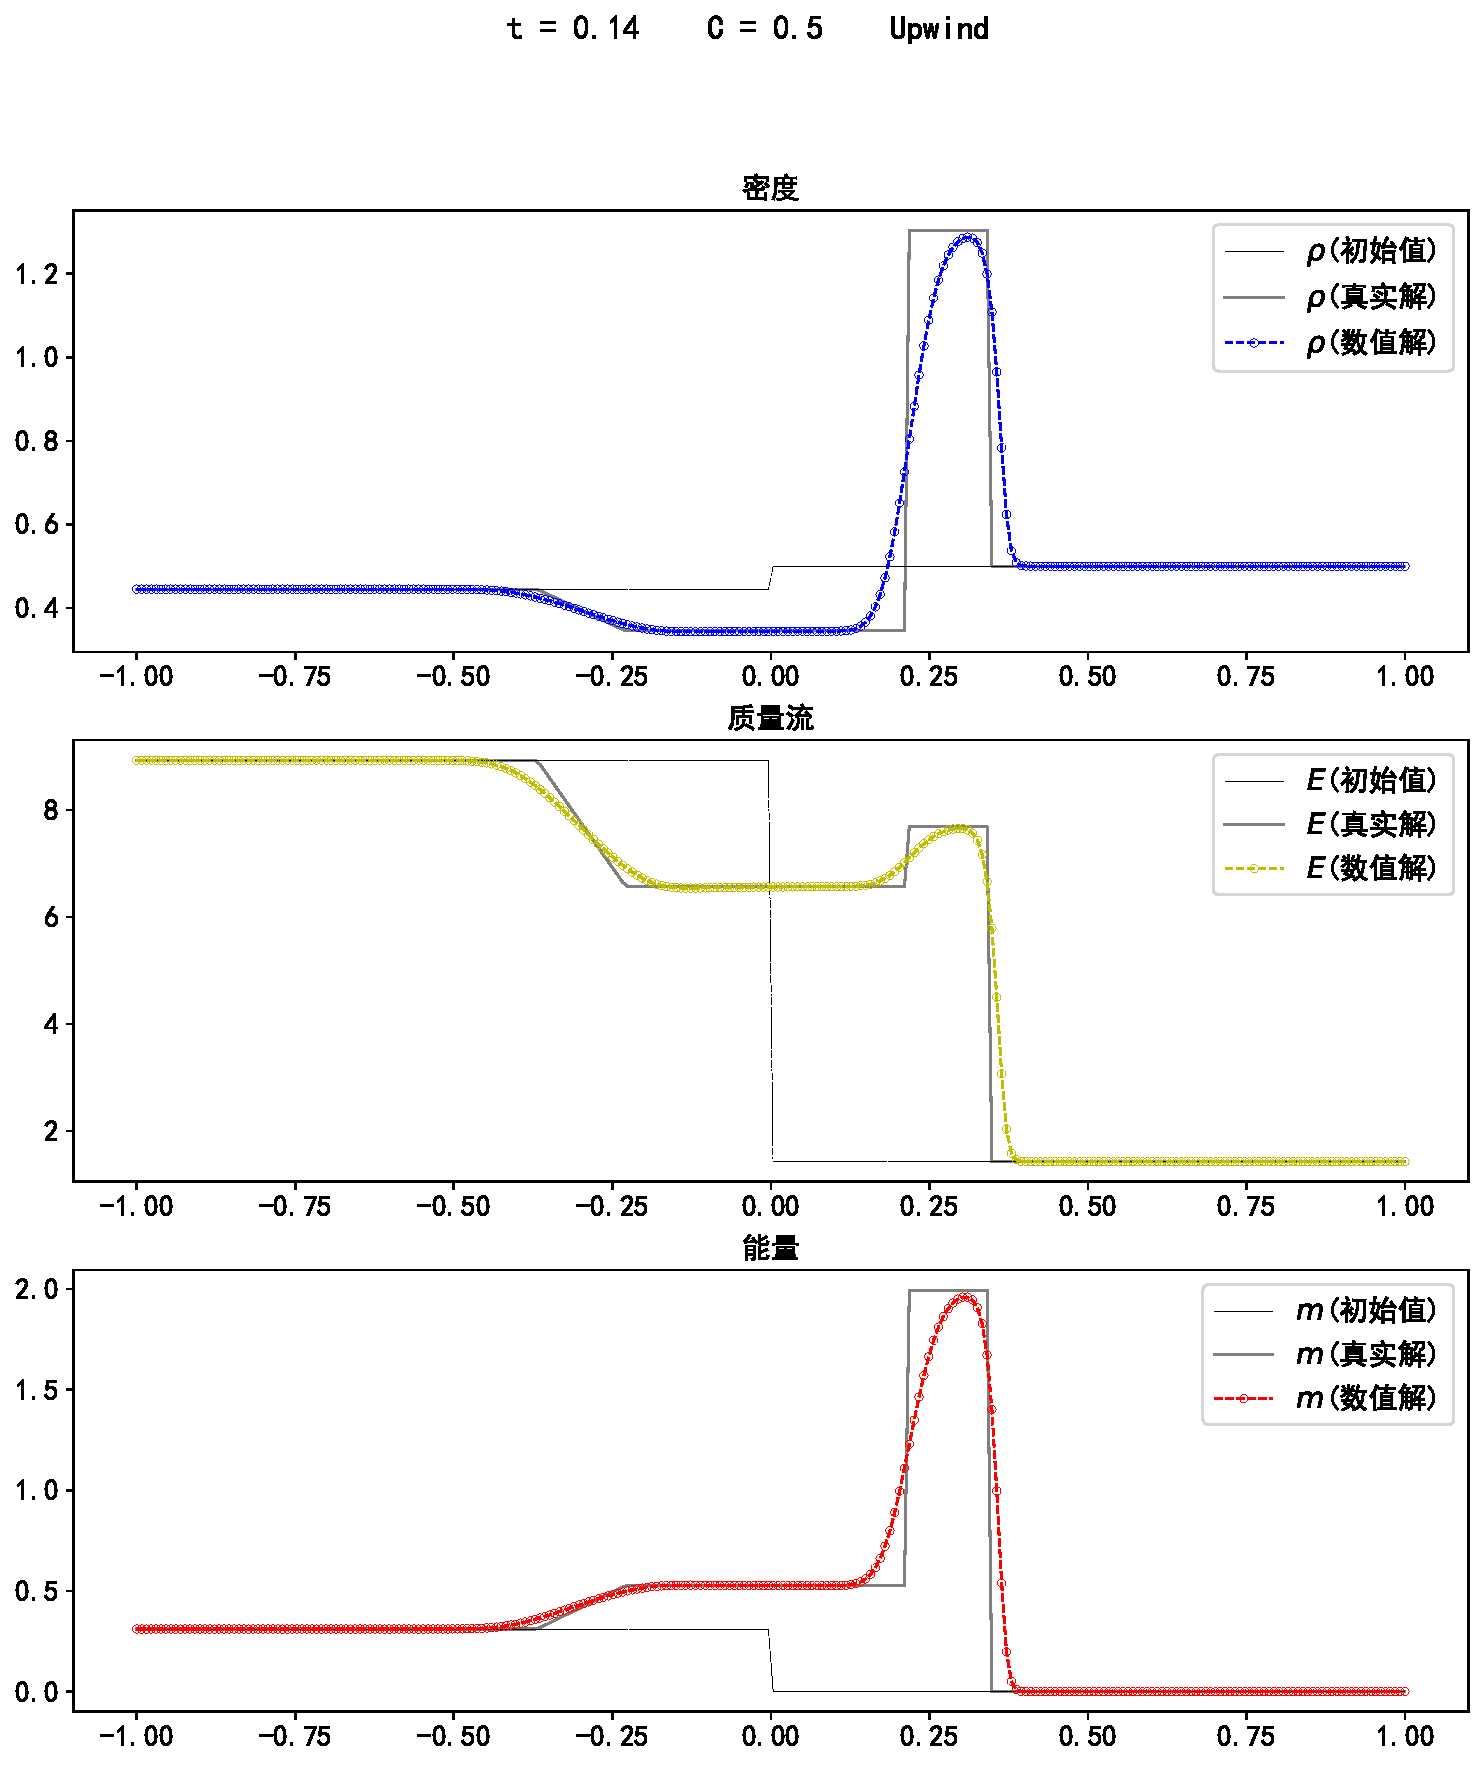
\includegraphics[width=.85\textwidth]{figures/upwind261.pdf}
\caption{迎风格式计算结果, 网格点数为 261. \textbf{从上到下分别是密度 $\rho$, 能量 $E$ 和质量流 $m = \rho u$.}
其中点线是初值, 虚线 (上面的数据点用符号 $\circ$ 标注) 是 $t=0.14$ 时的数值结果, 实线是对应的真实解.}\label{Fig:Upwind}
\end{center}
\end{figure}

\begin{figure}
\begin{center}
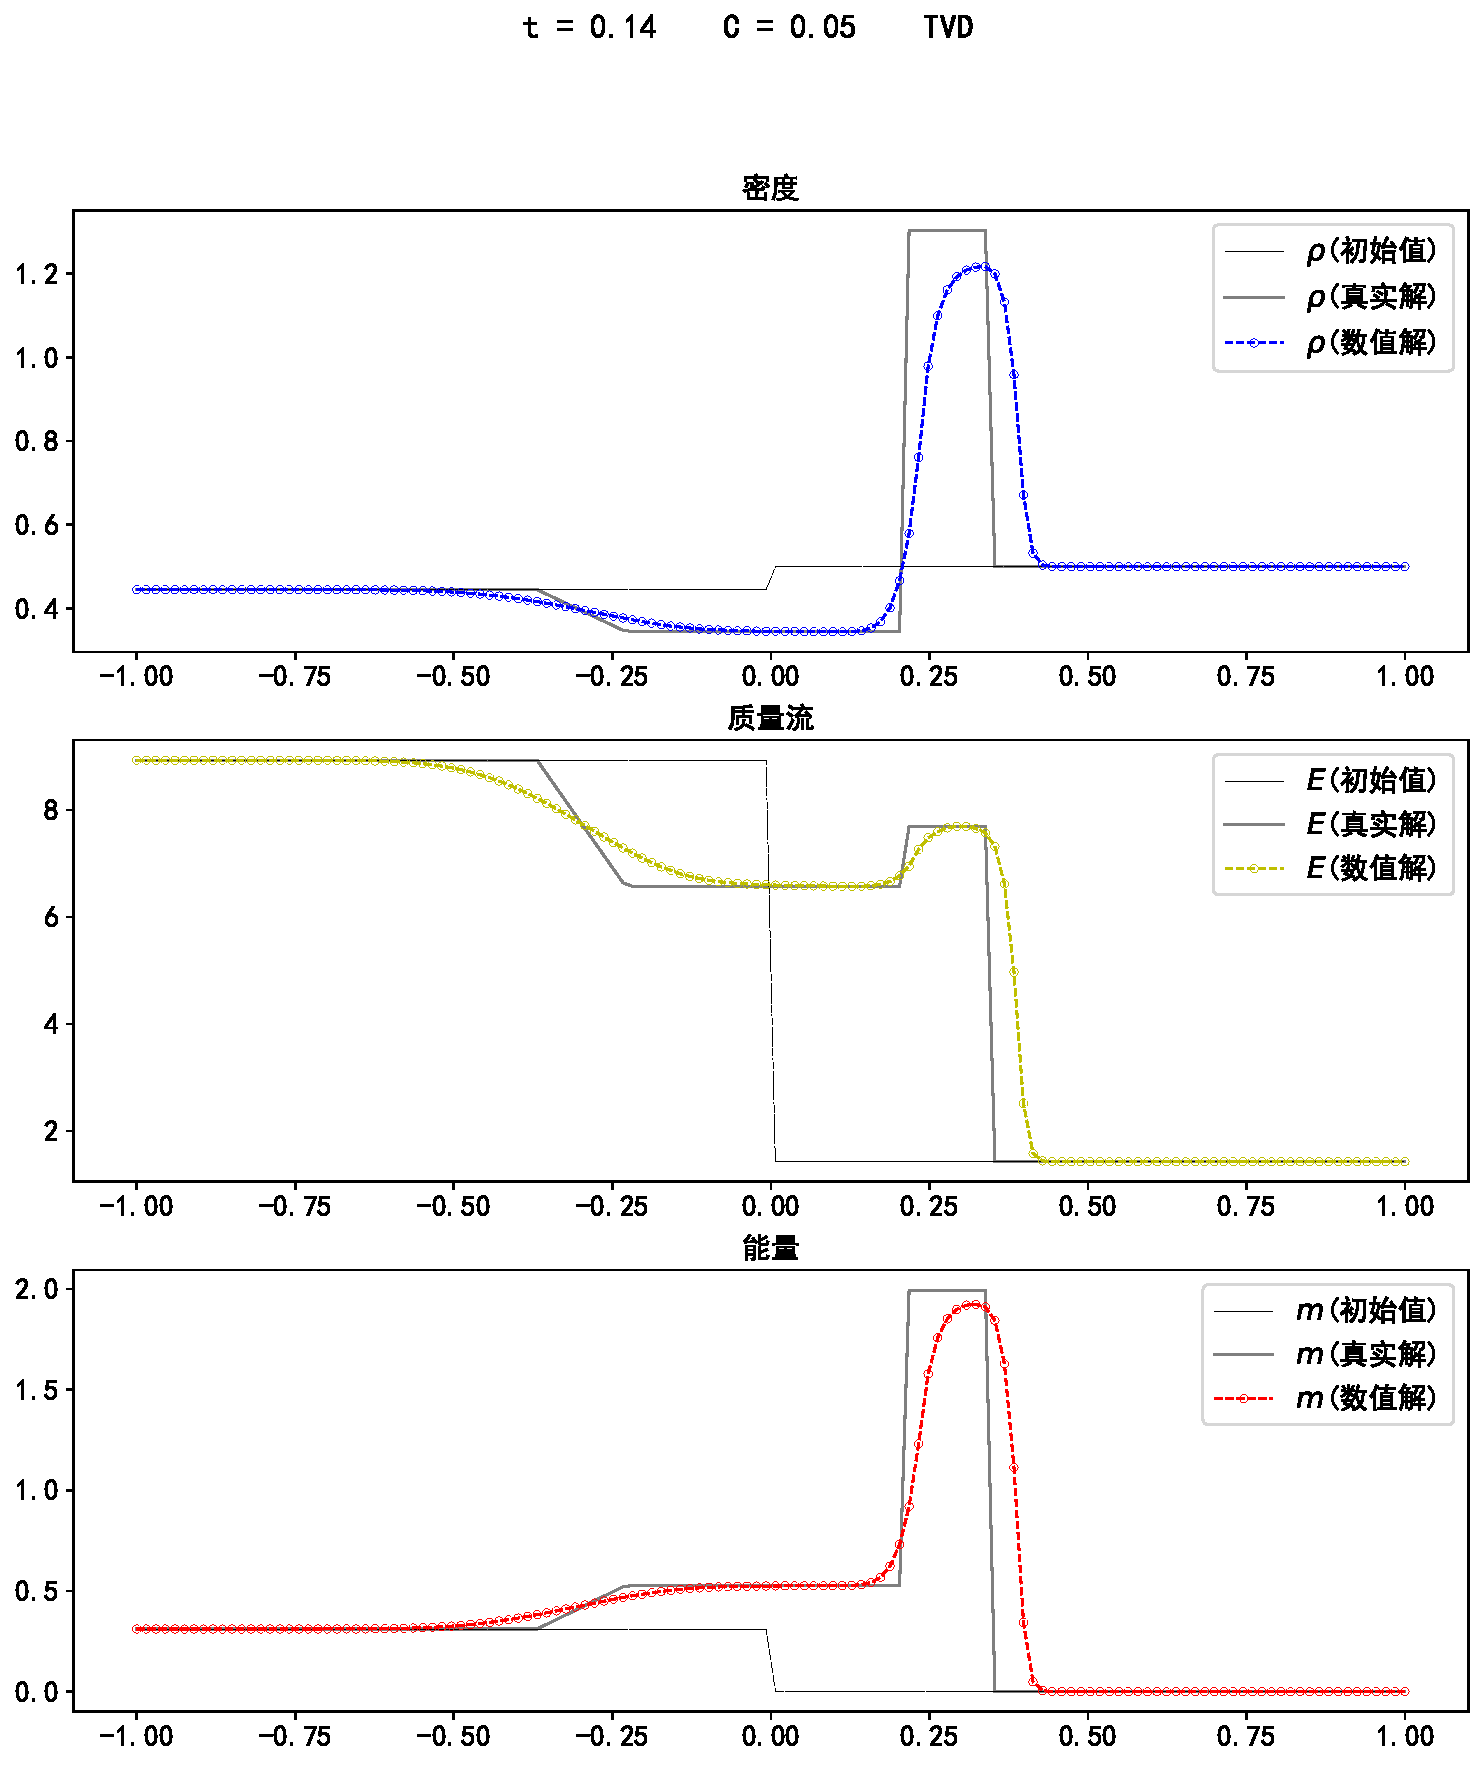
\includegraphics[width=.85\textwidth]{figures/limiter133.pdf}
\caption{(van Leer) TVD 格式计算结果, 网格点数为 133. 其他标注同图~\ref{Fig:Upwind}.}\label{Fig:vanLeerA}
\end{center}
\end{figure}

\begin{figure}
\begin{center}
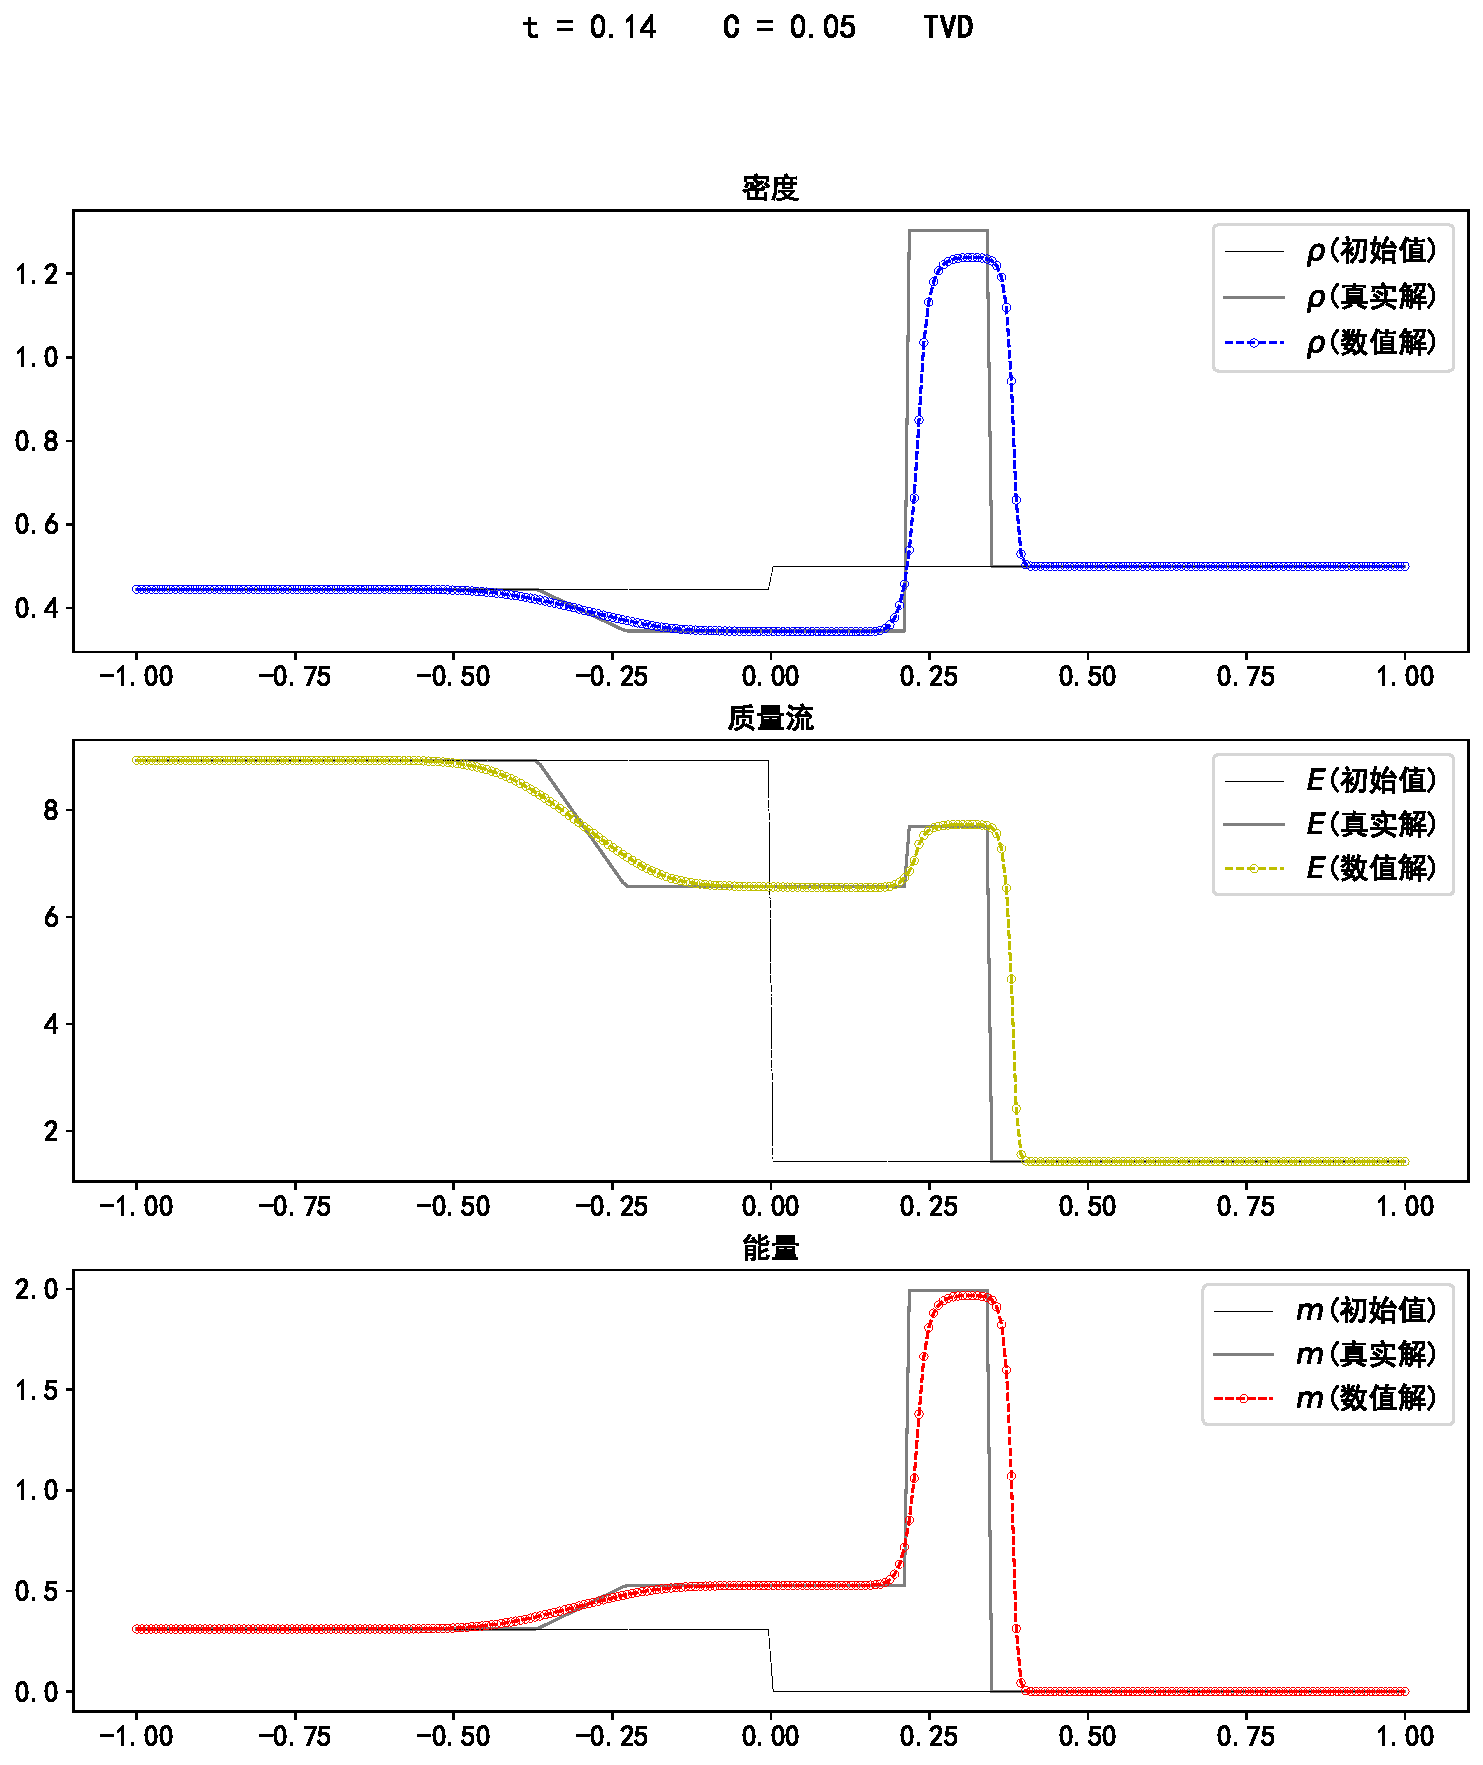
\includegraphics[width=.85\textwidth]{figures/limiter261.pdf}
\caption{(van Leer) TVD 格式计算结果, 网格点数为 261. 其他标注同图~\ref{Fig:Upwind}.}\label{Fig:vanLeerB}
\end{center}
\end{figure}

\section{格式参考}
\subsection{Lax-Wendroff格式}
对于守恒型方程,
\begin{align}
\frac{\partial u}{\partial t} + \frac{\partial F}{\partial x} = 0,
\end{align}
其 Lax-Wendroff 格式为
\begin{align}
u_j^{n+1} =& u_j^n - \frac{\Delta t}{2\Delta x} (F_{j+1}^n - F_{j-1}^n) \nonumber\\
& + \frac{\Delta t^2}{2\Delta x^2} \left[A_{j+1/2}^n (F_{j+1}^n-F_j^n) - A_{j-1/2}^n (F_j^n -
F_{j-1}^n)\right]
\end{align}
其中 $A = \frac{\partial F}{\partial u}$, $A$ 的表达式见第~\ref{Appendix}~节. 单元边界上的值可以取
\begin{align}
A_{j \pm 1/2}^n = A(u_{j \pm 1/2}^n), \qquad u_{j \pm 1/2}^n = \frac{1}{2} (u_j^n + u_{j \pm 1}^n)
\end{align}

\subsection{非守恒性 Upwind 格式}
式~(\ref{Eqn:Euler}) 的非守恒形式为
\begin{align}
\frac{\partial U}{\partial t} + A \frac{\partial U}{\partial x} = 0,
\end{align}
其中
\begin{align}
U = [u_j] = \left[\begin{array}{c}\rho\\ u\\ p\end{array}\right], \qquad A = A_{ij} = \left[\begin{array}{ccc}u & \rho & 0\\
0 & u & 1/\rho\\ 0 & \gamma p & u\end{array}\right]
\end{align}
矩阵 $A$ 的特征值为 $u-a$, $u$, $u+a$ ($a^2 = \gamma p/\rho$), 对应的左右特征向量矩阵为 $L$ 和 $R$ 写为
\begin{align}
L =& [L_{ij}] = \left[\begin{array}{ccc}0 & -\rho a & 1\\ a^2 & 0 & -1\\ 0 & \rho a & 1\end{array}\right],
\\
R =& [R_{ij}] = \left[\begin{array}{ccc}\frac{1}{2a^2} & \frac{1}{a^2} & \frac{1}{2a^2}\\
-\frac{1}{2\rho a} & 0 & \frac{1}{2\rho a}\\ \frac{1}{2} & 0 & \frac{1}{2}\end{array}\right]
\end{align}
波模分解的方程为
\begin{align}
\sum_j \left\{L_{ij} \frac{\partial u_j}{\partial t} + \lambda_i L_{ij} \frac{\partial u_j}{\partial
x}\right\} = 0,
\end{align}
其中
\begin{align}
\lambda_i =
\left[\begin{array}{c}u-a \\ u\\ u+a\end{array}\right]
\end{align}
在变换回原变量方程的形式, 即
\begin{align}
\sum_i \sum_j \left\{R_{ki} L_{ij} \frac{\partial u_j}{\partial t} + R_{ki} \lambda_i L_{ij}
\frac{\partial u_j}{\partial x}\right\} = 0,
\end{align}
并利用 $\sum_i R_{ki} L_{ij} = \delta_{kj}$, 我们有
\begin{align}
\frac{\partial u_k}{\partial t} + \sum_i \sum_j \left\{R_{ki} \lambda_i L_{ij} \frac{\partial
u_j}{\partial x}\right\} = 0,
\end{align}
迎风格式为
\begin{align}
u_{k,l}^{n+1} =& u_{k,l}^n \nonumber\\
& - \frac{\Delta t}{\Delta x} \sum_i \sum_j \left\{\text{sgn}(\lambda_{i,l}^n)
 \lambda_{i,l}^n R_{ki,l}^n L_{ij,l}^n \left[u_{j,l}^n - u_{j,l-\text{sgn}(\lambda_{i,l}^n)}^n\right]\right\}
\end{align}
其中下角标 $l$ 对应于空间格点位置, 其他下角标对应于分量.

\section{守恒形式方程的特征向量计算}\label{Appendix}
守恒形式下 $A$ 的表达式
\begin{align*}
A =& \frac{\partial f}{\partial w} = \left[\begin{array}{ccc} 0 & 1 & 0
\\
\frac{1}{2} (\gamma  - 3) u^2 & -(\gamma - 3) u & \gamma - 1
\\
(\gamma - 1) u^3 - \gamma \frac{u}{\rho} E & \gamma \frac{1}{\rho} E-\frac{3}{2} (\gamma
- 1) u^2 & \gamma u
\end{array}
\right]
\end{align*}
左右特征向量
\begin{align*}
R =& \left[\begin{array}{ccc} 1 & 1 & 1
\\
u - c & u & u + c
\\
H - u c & \frac{1}{2} u^2 & H + u c
\end{array}
\right]
\\
L =& \frac{\gamma - 1}{2 c^2} \left[\begin{array}{ccc} \frac{1}{2} u \left(u + \frac{2
c}{\gamma - 1}\right) & -\left(u + \frac{c}{\gamma - 1}\right) & 1
\\
2(H - u^2) & 2 u & - 2
\\
\frac{1}{2} u \left(u - \frac{2 c}{\gamma - 1}\right) & -\left(u - \frac{c}{\gamma -
1}\right) & 1
\end{array}
\right]
\end{align*}
其中
\begin{align*}
H =& \frac{E + p}{\rho} = \frac{c^2}{\gamma - 1} + \frac{1}{2} u^2,
\\
c^2 =& \gamma \frac{p}{\rho}.
\end{align*}

\section{分工说明}

郑惠南提供了最初的报告文本, 数值计算结果生成的图形文件. 高新亮对整个文档结构, 规范, 文件清单进行了检查, 确认.

\section{附件}

\begin{enumerate}
\item
assign3.tex--本报告 \LaTeX  文件.
\item
assign3.pdf--本报告 PDF 输出文件.
\item
References.bib -- 文献文件
\item
GasUpwind261.eps--迎风格式计算结果, 261 网格.
\item
GasvanLeer133.eps--van Leer TVD 格式计算结果, 133 网格.
\item
GasvanLeer261.eps--van Leer TVD 格式计算结果, 261 网格.
\item
Hydrodynamics.xlsx--相关问题 Excel 计算表格, 深绿色单元为输入, 可以变更, 供大家参考. 其中
\begin{enumerate}
\item
  Riemann 表格中, B2 为 $\gamma$ 值, B4--B6 和 E4--E6 分别是左侧和右侧的密度, 质量流及能量的初值. A25--A26 迭代用值, A24 为 A25 和 A26 的平均值.
  22 行复制 24 行的值. 当 G24, 即 G22 值为零时, 得到此 Riemann 问题的解. N3 为时间值, 密度, 质量流及能量图形的坐标初值和对应比例分别由 N4--N6 和 O4--O6 调节.
\item
Hydrodynamics 表格为对应守恒型方程的矩阵特征值, 左右特征向量, 变量在各个波模的分解, 等等. 这些可以用于检查后续高精度格式计算的一些中间结果是否正确.
\end{enumerate}
\end{enumerate}

\bibliographystyle{apalike}
\bibliography{References}

\end{document}
